\documentclass[12pt]{article}
\usepackage{amsmath, amssymb,amsthm,enumerate,bm}
\usepackage{hyperref}
\usepackage{cite}
\usepackage{listings}
\usepackage{pdfpages}

\usepackage[a4paper,bindingoffset=0.2in,%
left=0.8in,right=0.8in,top=1in,bottom=1in,%
footskip=.25in]{geometry}

\DeclareMathOperator*{\argmin}{argmin}
\newcommand{\ttt}[1]{\textbf{#1}}
\newcommand{\la}{\langle}
\newcommand{\ra}{\rangle}
\newcommand{\ip}[4]{\langle \textbf{#1}_{#2} , \textbf{#3}_{#4} \rangle}

\title{Advanced Methods Homework 1}
\date{\today}
\author{Bohao Tang}

\begin{document}

\maketitle

\section{Vector spaces and inner products}
\begin{enumerate}
   \item
   \begin{proof}
        Denote $\{\textbf{a}_1,\textbf{a}_2,\cdots,\textbf{a}_k\}$ be a basis of $W$.
        And we can expand them to a basis of $\mathbb{R}^n$ as $\{\textbf{a}_1,\textbf{a}_2,\cdots,\textbf{a}_k,\textbf{a}_{k+1},\cdots,\textbf{a}_n\}$.
        Then we do Gram-Schmidt orthogonalization to the basis and get 
        $\{\textbf{b}_1,\textbf{b}_2,\cdots,\textbf{b}_k,\textbf{b}_{k+1},\cdots,\textbf{b}_n\}$.
        It's easy to see that $\{\textbf{b}_1,\textbf{b}_2,\cdots,\textbf{b}_k\}$ become an othogonal basis of $W$
        (they are othogonal, hence linear independent, and $k$ is the dimension of $W$).
        Now we assert that $V = $ \textbf{span}$\{\textbf{b}_{k+1},\cdots,\textbf{b}_n\}$ will be $W^\bot$.
       
        First, for every vector $\textbf{x}$ in $W^\bot$, it has a representation $\textbf{x} = \sum_{i=1}^n \omega_i \textbf{b}_i$ for some $\omega_i \in \mathbb{R}^n$.
        Since $\textbf{x} \in W^\bot$, we have $\langle \textbf{x} , \textbf{b}_j \rangle = 0$, for all $j = 1,2,\cdots,k$.
        Therefore $\omega_j = 0$ for $1 \le j \le k$, which means $\textbf{x} \in V$ and $W^\bot \subset V$.
        
        In the other side, for every vector $\textbf{y} = \sum_{t=k+1}^n \gamma_t \textbf{b}_t \in V$, it's quite direct to see that $\langle \textbf{y} , \textbf{b}_j \rangle = 0$, for all $j = 1,2,\cdots,k$,
        hence $\langle \textbf{y} , \textbf{w} \rangle = 0$, for all $\textbf{w} \in W$.
        Therefore $\textbf{y} \in W^\bot$ and $W^\bot \subset V$.

        Now we get $W^\bot = V$, hence dim$(W^\bot) = n-k$. Also we can see that $W^\bot$ is unique. 
        If not, we can merge the two different $W^\bot$ and get a higher dimensional subspace $Z$ that is orthogonal to $W$.
        Then $Z \oplus W \subset \mathbb{R}^n$ but dim$(Z \oplus W) \ge n+1 > n$, a contradiction. 
    \end{proof}
    \item
    \begin{enumerate}[(a)]
        \item 
        \begin{proof}
            According to Cauchy inequality, $\left(\sum u_i v_i\right)^2 \le \sum u_i^2 \sum v_i^2$. It's equivalent here that $|\langle \textbf{u}, \textbf{v} \rangle| \le ||\textbf{u}|| ||\textbf{v}||$.
        \end{proof}
        \item
        \begin{proof}
            \begin{align}
                ||\textbf{u} + \textbf{v}||^2 + ||\textbf{u} - \textbf{v}||^2 &= (\textbf{u} + \textbf{v})'(\textbf{u} + \textbf{v}) + (\textbf{u} - \textbf{v})'(\textbf{u} - \textbf{v}) \\
                                                                              &= \textbf{u}'\textbf{u} + 2 \textbf{u}'\textbf{v} + \textbf{v}'\textbf{v} + \textbf{u}'\textbf{u} - 2 \textbf{u}'\textbf{v} + \textbf{v}'\textbf{v} \\
                                                                              &= 2 \textbf{u}'\textbf{u} + 2 \textbf{v}'\textbf{v} = 2 ||\textbf{u}||^2 + 2 ||\textbf{v}||^2
            \end{align}
        \end{proof}
    \end{enumerate}
    \item
    In the definition of projection in Lecture 2, $\textbf{y - $\Pi$(y|x)}$ should be orthogonal to $\textbf{x}$. So there is nothing need to be proved. 
    Maybe we should changed the definition here that (suppose $\textbf{x} \neq \textbf{0}$, or there is no meaningful projection)
    $$\Pi\textbf{(y|x)} \triangleq \argmin_{\textbf{u} \in \text{span}\{\textbf{x}\}} ||\textbf{y - u}||^2$$
    \begin{proof}
        (This proof contains the part to assert that projection above is well defined)
        Suppose $\textbf{u} = b \textbf{x}$, then $||\textbf{y} - \textbf{u}||^2 = \textbf{y}'\textbf{y} - 2 b \textbf{x}'\textbf{y} + b^2 \textbf{x}'\textbf{x}$.
        It's a quadratic function with highest coefficient $\textbf{x}'\textbf{x} > 0$, therefore have a unique minimizer.
        Differentiate it with $b$, let it be zero and we get the normal equation $\textbf{x}'\textbf{y} = b \textbf{x}'\textbf{x}$,
        which means (since $\Pi(\textbf{y|x}) = b \textbf{x}$) : $\langle \Pi(\textbf{y|x}), x \rangle = \langle \textbf{y}, x \rangle$ and therefore $\textbf{y} - \Pi(\textbf{y|x}) \  \bot \ \textbf{x}$.
    \end{proof}
\end{enumerate}

\section{Regression}

\begin{enumerate}
    \item 
    Slope $\hat{\beta}_{yx}$ of regressing \textbf{y} on \textbf{x} is $\hat{\rho}_{xy}\ \frac{\hat{\sigma}_y}{\hat{\sigma}_x}$, where $\hat{\rho}_{xy}$ is the sample correlation coefficient and $\hat{\sigma}_y, \hat{\sigma}_x$ are the sample standard deviation of $y$ and $x$.
    So, slope $\hat{\beta}_{xy}$ of \textbf{x} on \textbf{y} is $\hat{\rho}_{yx}\ \frac{\hat{\sigma}_x}{\hat{\sigma}_y}$.
    We have that $\hat{\rho}_{xy} = \hat{\rho}_{yx}$, so $\hat{\beta}_{xy} \hat{\beta}_{yx} = \hat{\rho}_{xy}^2$.
    \item
    \begin{proof}
        In the setting of mean only regression of \textbf{y}, we have $\hat{\mu} = \overline{\textbf{y}} = \sum_{i=1}^n y_i / n$.
        And the residual is $\textbf{r} = \textbf{y} - \overline{\textbf{y}} \textbf{J}_n$, therefore sum of residual is $\sum r_i = \sum_1^n y_i - n \cdot \sum_1^n y_i / n = 0$.
    \end{proof}
    \item
    \begin{proof}
        In the setting of mean only regression of \textbf{y} on \textbf{x}, we have $\hat{\beta} = \frac{\langle \textbf{y}, \textbf{x} \rangle}{\langle \textbf{x}, \textbf{x} \rangle}$.
        Therefore residual is $\textbf{r} = \textbf{y} - \frac{\langle \textbf{y}, \textbf{x} \rangle}{\langle \textbf{x}, \textbf{x} \rangle} \textbf{x}$, therefore $\langle \textbf{r}, \textbf{x} \rangle = \langle \textbf{y}, \textbf{x} \rangle - \frac{\langle \textbf{y}, \textbf{x} \rangle}{\langle \textbf{x}, \textbf{x} \rangle}\cdot\langle \textbf{x}, \textbf{x} \rangle = 0$, $\textbf{r} \bot \textbf{x}$.
    \end{proof}
    \item
    Notation as above, when $\textbf{y} \bot \textbf{x}$, we find that the residual $\textbf{r} = \textbf{y}$, which of course need not sum to zero.
    \item
    \begin{proof}
        In this setting of regressing \textbf{y} on \textbf{x}, we get the normal equation that:
        \begin{eqnarray}
            \textbf{J}_n'\textbf{y} &=& \hat{\beta}_0 \textbf{J}_n'\textbf{J}_n + \hat{\beta}_1 \textbf{J}_n'\textbf{x} \\
            \textbf{x}'\textbf{y} &=& \hat{\beta}_0 \textbf{x}'\textbf{J}_n + \hat{\beta}_1 \textbf{x}'\textbf{x}
        \end{eqnarray} 
    and also the residual $\textbf{r} = \textbf{y} - \hat{\beta}_0 \textbf{J}_n - \hat{\beta}_1 \textbf{x}$.
    Then: 
    $$\langle \textbf{r}, \textbf{J}_n \rangle = \textbf{J}_n'\textbf{y} - \hat{\beta}_0 \textbf{J}_n'\textbf{J}_n + \hat{\beta}_1 \textbf{J}_n'\textbf{x} = 0$$
    and
    $$\langle \textbf{r}, \textbf{x} \rangle = \textbf{x}'\textbf{y} - \hat{\beta}_0 \textbf{x}'\textbf{J}_n + \hat{\beta}_1 \textbf{x}'\textbf{x} = 0$$
    So we get the residual $\textbf{r} \bot \textbf{J}_n$ and $\textbf{r} \bot \textbf{x}$.
    \end{proof}
\end{enumerate}

\section{Least squares}

\begin{enumerate}
    \item
    \begin{proof}
        Given $\textbf{H}^2 = \textbf{H}$, then $\textbf{(I - H)}^2 = \textbf{I}^2 - 2 \textbf{H} + \textbf{H}^2 = \textbf{I} - 2 \textbf{H} + \textbf{H} = \textbf{I - H}$.
    \end{proof}
    \item
    After calculating, I think the method mentioned to estimate $\beta_2$ in this question is:
    \begin{itemize}
        \item First, regressing $\ttt{y}$ on $\ttt{x}_1$ through origin and get the residual $\ttt{r}_1$.
        \item Second, regressing $\ttt{x}_2$ on $\ttt{x}_1$ through origin and get the residual $\ttt{r}_2$.
        \item Finally, regressing $\ttt{r}_1$ on $\ttt{r}_2$ through origin and get the estimation $\hat{\beta}_2$.
    \end{itemize}
    \begin{proof}
        To minimize $||\ttt{y} - \beta_1 \ttt{x}_1 - \beta_2 \ttt{x}_2||^2$, we can first suppose $\beta_2$ be a constant and minimize through $\beta_1$(it will be a function of $\beta_2$), and then minimize through $\beta_2$ to get the estimation.
        So the goal is firstly to find the $\argmin_{\beta_1} ||(\ttt{y} - \beta_2 \ttt{x}_2) - \beta_1 \ttt{x}_1||^2$. This is simply a regression through origin and we can get that
        $\beta_1^{min} = \frac{\la \ttt{y} - \beta_2 \ttt{x}_2, \ttt{x}_1 \ra}{\la \ttt{x}_1, \ttt{x}_2 \ra}$.

        Therefore, the second step is to find the argmin of:
        $$ ||\ttt{y} - \beta_2\ttt{x}_2 - \frac{\la \ttt{y} - \beta_2 \ttt{x}_2, \ttt{x}_1 \ra}{\la \ttt{x}_1, \ttt{x}_2 \ra} \ttt{x}_1||^2 = ||(\ttt{y} - \frac{\la \ttt{y}, \ttt{x}_1 \ra}{\la \ttt{x}_1, \ttt{x}_1 \ra}\ttt{x}_1) - \beta_2 (\ttt{x}_2 - \frac{\la \ttt{x}_2, \ttt{x}_1 \ra}{\la \ttt{x}_1, \ttt{x}_1 \ra} \ttt{x}_1)||^2$$
        Also, we can find that:
        \begin{eqnarray}
            \ttt{r}_1 &=& \ttt{y} - \frac{\la \ttt{y}, \ttt{x}_1 \ra}{\la \ttt{x}_1, \ttt{x}_1 \ra}\ttt{x}_1\\
            \ttt{r}_2 &=& \ttt{x}_2 - \frac{\la \ttt{x}_2, \ttt{x}_1 \ra}{\la \ttt{x}_1, \ttt{x}_1 \ra} \ttt{x}_1
        \end{eqnarray}
        Therefore, $\hat{\beta}_2$ comes from minimizing $||\ttt{r}_1 - \beta_2 \ttt{r}_2||^2$, which is just doing regression through origin of $\ttt{r}_1$ on $\ttt{r}_2$.
        Then we finish the proof that the procedure described in the question is valid.
    \end{proof}
    \item
    \begin{proof}
        Suppose that $\ttt{X}$ is of size $m \times n$, where $m \le n$ (or we replace $\ttt{X}$ by $\ttt{X}'$, and we just need to prove the same thing).
        Then consider the singular value decomposition of $\ttt{X}$ is $\ttt{X} = \ttt{U} \ttt{S} \ttt{V}$,
        where $\ttt{U},\ttt{V}$ are orthogonal matrices and $\ttt{S} = \left( diag\{\lambda_1,\lambda_2,\cdots,\lambda_r,0,\cdots,0\}, \ttt{0} \right): \  \lambda_1 \ge \lambda_2 \ge \lambda_3 \ge \cdots \ge \lambda_r > 0$.
        Here $r = rank(\ttt{X})$. Now consider the svd of $\ttt{X}', \ttt{X}'\ttt{X}, \ttt{X}\ttt{X}'$, we have:
        \begin{eqnarray}
            \ttt{X}' &=& \ttt{V}' \ttt{S}' \ttt{U}'\\
            \ttt{X}'\ttt{X} &=& \ttt{V}' \begin{pmatrix} 
                                            diag\{\lambda_1^2,\lambda_2^2,\cdots,\lambda_r^2,0,\cdots,0\} & \ttt{0} \\
                                            \ttt{0} & \ttt{0} 
                                         \end{pmatrix} \ttt{V} \\
            \ttt{X}\ttt{X}' &=& \ttt{U}\ diag\{\lambda_1^2,\lambda_2^2,\cdots,\lambda_r^2,0,\cdots,0\}\ \ttt{U}'
        \end{eqnarray}
        Therefore we can see that the three matrices above all have and only have $r$ nonzero singular values, which means they are all of rank $r$.
        Then we get $rank(\ttt{X}) = rank(\ttt{X}') = rank(\ttt{X}'\ttt{X}) = rank(\ttt{X}\ttt{X}')$.
    \end{proof}
    \item
    If the design matrix is orthogonal, then we have:
    $$\ttt{J} = ||\ttt{y} - \ttt{X}\bm{\beta}||^2 = \ttt{y}'\ttt{y} - 2 \ttt{y}'\ttt{X}\bm{\beta} + \bm{\beta}' \ttt{X}'\ttt{X} \bm{\beta} = \ttt{y}'\ttt{y} - 2 \ttt{y}'\ttt{X}\bm{\beta} + \bm{\beta}'\bm{\beta}$$
    And then we get the normal equation as:
    $$\frac{\partial \ttt{J}}{\partial \bm{\beta}} = 2 \bm{\beta} - 2 \ttt{X}'\ttt{y} = 0$$
    So we have $\hat{\bm{\beta}} = \ttt{X}'\ttt{y}$. 
\end{enumerate}

\section{Computing and analysis}
Code is shown below and we simulate the data ourselves and test the $L_1$ norm of the differences of $\hat{\beta}$, fitted\_value and residuals from two results. 

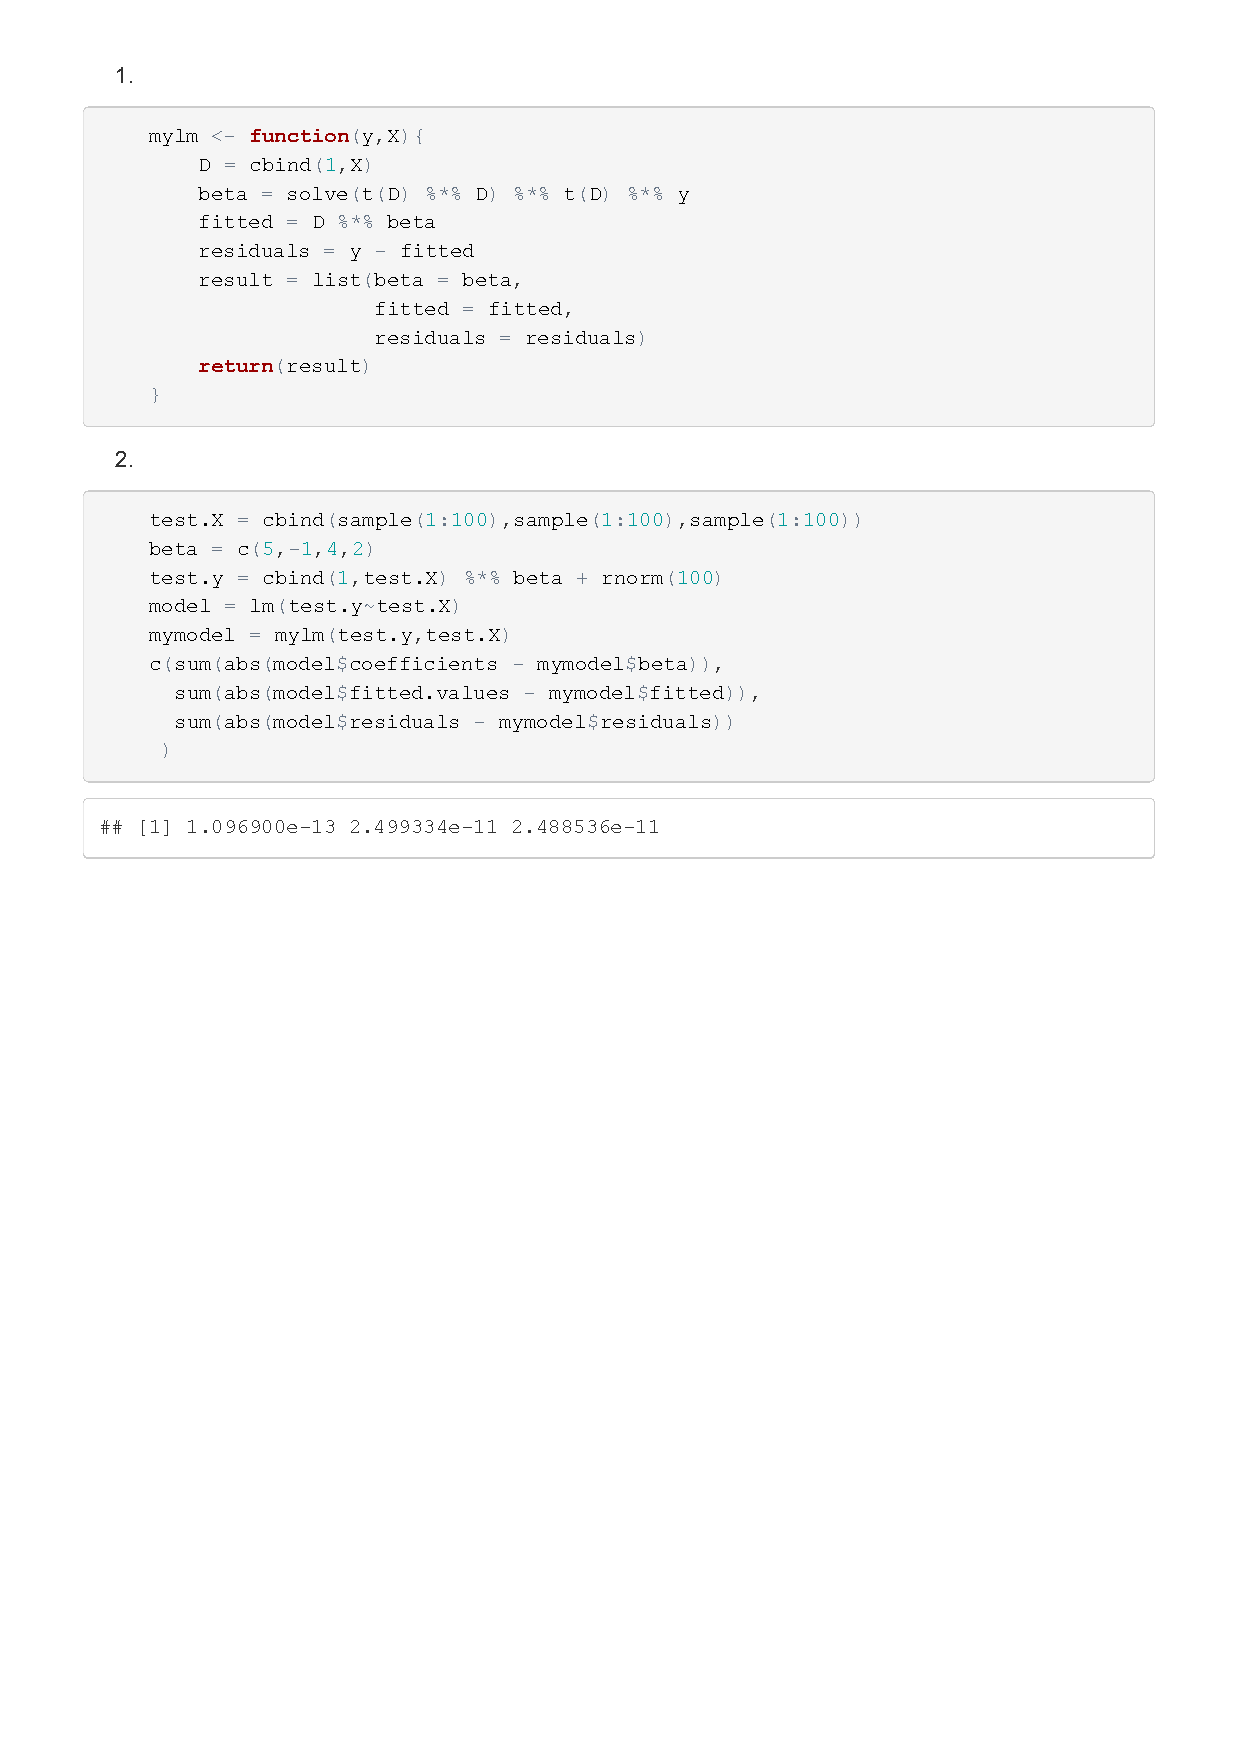
\includepdf[pages=-]{rcode.pdf}

\end{document}